\section{Software Design}

\paragraph{}
The majority of the scope of this project was related to the software and firmware design and implementation.
This section details the design of the software, it's implementation, as well as issues encountered and the ways in which they were addressed or what needs to happen to address the issue.

\subsection{High Level Design and Implementation}

\paragraph{}
The software for this DAQ is designed and implemented to be run in a pseudo-parallel manner.
This means that there are several different tasks that are running sequentially, with each task running small chunks or sub-tasks during each cycle.
Each task is then designed as a state machine to segment itself into these smaller sub-tasks.
In order for each of these tasks to communicate with each other, there is one group of data that each task can reference.
Since this is a sequential action still, conflicts will not occur and ther does not need to be any extra protections for accessing the same data or variable at the same time.

\paragraph{}
The DAQ runs four main tasks that are continuously cycled through:
\begin{itemize}
	\item[(1)] Storage
	\item[(2)] Communication
	\item[(3)] Radio Communication
	\item[(4)] Sensors
	\item[(5)] Health Monitoring
\end{itemize}
The storage task is responsible for the actual logging of data.
The communication task is the task responsible for reading data off the CAN bus.
The radio communication task is responsible for medium-long range telemetry.
The sensors task is responsible for the reading of all on-board sensors.
The health monitoring task is responsible for updating any LED indicators for the health of the system.
Together, these five main tasks handle the running of all parts of the system.
As can be seen in \cref{fig:SoftwareTasks}, these tasks all run sequentially before looping back to the start.

\begin{figure}[H]
	\centering
	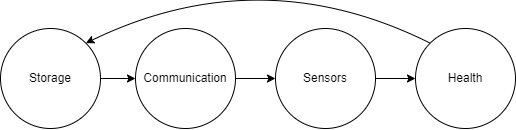
\includegraphics[width=\linewidth]{SoftwareTasks.png}
	\caption{Software tasks loop diagram}
	\label{fig:SoftwareTasks}
\end{figure}

\paragraph{}
Object-oriented programming (OOP) is utilized significantly for this design.
Every task and sensor is a class that have individiual constructors depending on the needs of the task.
Additionally, each task gets its own enum classes to define the various states for each state machine.
There are two parent classes that are utilized by everything.
For different tasks, there is an abstract task class that forces an implementation for a function that runs the task and requires the intercommunication data to be passed in.
For sensors, there is an abstract sensor class that forces an implementation for two functions, an initialization function and an update function.
Additionally, this class implements a read function that returns the current sensor value.

\paragraph{}
Since this project is based on the Arduino platform, several of the basic tasks for interacting with the hardware are handled by the platform.
This includes things such as setting the mode of a pin, reading and writing from data registers, configuring UART, SPI, and SDIO interfaces, and configuring the interrupt vector table.
Even with the configuration of these periphreals being handled by Arduino, they still need to be configured with the proper settings to be used.
Despite all falling under the Arduino umbrella, each platform is maintained independently of each other.
The people maintaining the Arduino platform for Teensy and the people maintaining the Arduino platform for STM do not communicate with each other, and as a result there are some implementation differences that exist between different hardware platforms using Arduino.

\paragraph{}
Additionally, not every family of microcontrollers from STM receives the same support or even the sample supported functions from the Arduino framework.
One specific issue that arose was a versioning issue for STM32duino.
In versions 18.0.0 onwards, the memory sizes of the H7 family of STM microcontrollers was updated incorrectly, causing code to not run and the debugger to be unusable.
This issue was resolved by reverting the version of STM32duino back to 17.6.0.
Other issues that arose that were not issus on the Teensy platform were the signedness of pins on the STM32, multiple timers on the same timer channels, timer registers having different sizes, and the same interrupt being tied to multiple pins.
One of the largest benefits of this change was having access to the debugger.
Without access to a deebugger, many of these issues would not have been solved or would have taken weeks or longer to debug.

\subsection{Storage Task}

\paragraph{}
The first and foremost task that the DAQ runs is the storage task.
This task is responsible for managing the SD interface as well as managing the filesystem.
This includes things like initializing the communication interface with the SD card, setting up the filesystem, and writing data to the SD card.